\documentclass[12pt,a4paper]{article}

% ============================================================================
% PACKAGES
% ============================================================================
\usepackage[utf8]{inputenc}
\usepackage[T1]{fontenc}
\usepackage{lmodern}
\usepackage[margin=2.8cm]{geometry}
\usepackage{amsmath,amssymb,amsthm}
\usepackage{xcolor}
\usepackage{tikz}
\usepackage{hyperref}
\usepackage{fancyhdr}
\usepackage{titlesec}
\usepackage{lettrine}
\usepackage{setspace}
\usepackage{parskip}
\usepackage{epigraph}
\usepackage{enumitem}
\usepackage{microtype}
\usepackage{abstract}

% ============================================================================
% CONFIGURATION
% ============================================================================
\usetikzlibrary{decorations.pathmorphing, decorations.markings, arrows.meta, calc, patterns, fadings}

% Colors
\definecolor{voidblack}{RGB}{10, 10, 20}
\definecolor{deepblue}{RGB}{20, 60, 120}
\definecolor{quantumblue}{RGB}{70, 130, 200}
\definecolor{starwhite}{RGB}{255, 255, 240}
\definecolor{nebula}{RGB}{150, 100, 180}
\definecolor{fieldgreen}{RGB}{80, 180, 140}
\definecolor{amber}{RGB}{200, 150, 50}
\definecolor{cosmicred}{RGB}{180, 60, 60}

\hypersetup{
    colorlinks=true,
    linkcolor=deepblue,
    citecolor=nebula,
    urlcolor=quantumblue,
    pdftitle={The Eternal Ledger: On the Philosophical Significance of a Medium That Never Resets},
    pdfauthor={Q-NarwhalKnight Research Group}
}

% Header/Footer
\pagestyle{fancy}
\fancyhf{}
\fancyhead[LE,RO]{\small\thepage}
\fancyhead[RE]{\small\textit{The Eternal Ledger}}
\fancyhead[LO]{\small\textit{Q-NarwhalKnight Research}}
\renewcommand{\headrulewidth}{0.4pt}

% Title formatting
\titleformat{\section}{\Large\bfseries\color{deepblue}}{\thesection}{1em}{}[\vspace{-0.5em}\color{deepblue}\rule{\textwidth}{0.3pt}]
\titleformat{\subsection}{\large\bfseries\color{nebula}}{\thesubsection}{1em}{}
\titleformat{\subsubsection}{\normalsize\itshape\color{amber}}{\thesubsubsection}{1em}{}

% Spacing
\setstretch{1.35}

% Epigraph settings
\setlength{\epigraphwidth}{0.8\textwidth}
\setlength{\epigraphrule}{0pt}

% Theorem environments
\newtheoremstyle{philosophical}%
  {12pt}{12pt}{\itshape}{0pt}{\bfseries\color{deepblue}}{.}{.5em}{}
\theoremstyle{philosophical}
\newtheorem{thesis}{Thesis}
\newtheorem{observation}{Observation}
\newtheorem{principle}{Principle}
\newtheorem{meditation}{Meditation}

% ============================================================================
% DOCUMENT
% ============================================================================
\begin{document}

% ============================================================================
% TITLE PAGE
% ============================================================================
\begin{titlepage}
\begin{center}

\vspace*{2cm}

% Decorative element
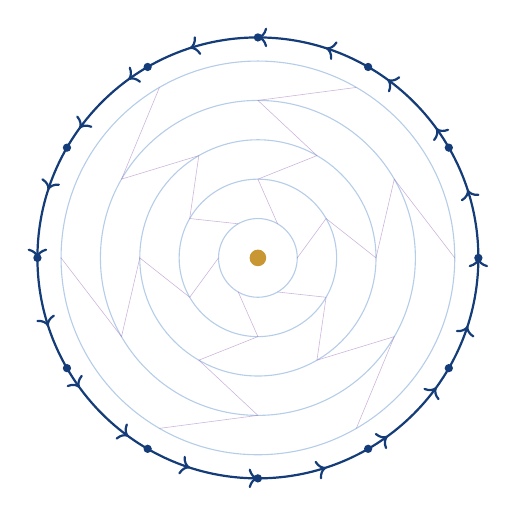
\begin{tikzpicture}[remember picture]
  % Outer ring - the eternal cycle
  \draw[deepblue, thick, decoration={markings, mark=between positions 0 and 1 step 0.05 with {\arrow{>}}}, postaction={decorate}] (0,0) circle (2.8cm);
  % Inner ring - the growing medium
  \foreach \r in {0.5, 1.0, 1.5, 2.0, 2.5} {
    \draw[quantumblue!40, thin] (0,0) circle (\r cm);
  }
  % Vertices on the DAG
  \foreach \a in {0,30,...,330} {
    \fill[deepblue] (\a:2.8) circle (1.5pt);
  }
  % Connections - the growing past
  \foreach \a in {0,60,...,300} {
    \draw[nebula, very thin, opacity=0.5] (\a:0.5) -- (\a+30:1.0) -- (\a:1.5) -- (\a+30:2.0) -- (\a:2.5);
  }
  % Center point - the present
  \fill[amber] (0,0) circle (3pt);
\end{tikzpicture}

\vspace{1.5cm}

{\fontsize{28}{34}\selectfont\bfseries\color{deepblue} The Eternal Ledger}

\vspace{0.6cm}

{\Large\color{nebula}\textit{On the Philosophical Significance of a Medium\\[4pt] That Never Resets, Only Grows}}

\vspace{1.2cm}

{\large Q-NarwhalKnight Research Group}\\[6pt]
{\normalsize\texttt{research@quillon.xyz}}

\vspace{0.8cm}

{\normalsize Version 1.0 --- February 2026}

\vspace{2cm}

\begin{abstract}
\noindent
We present a philosophical investigation into the ontological, epistemological, and ethical implications of a computational medium that, by mathematical construction, can never be reset---only extended. Drawing upon the quantum field-theoretic framework of the Q-NarwhalKnight consensus system, where the Consensus Hamiltonian $\mathcal{H}_{\mathrm{DAG}}$ admits only monotonically growing ground states, we argue that such a medium constitutes a fundamentally new category of being: an \emph{artificial memory} that is neither biological nor geological, yet shares with both the property of irreversible temporal accumulation. We explore the connections between the DAG's arrow of time and the Second Law of Thermodynamics, the philosophical status of a ``ledger of everything,'' the ethics of permanence in an impermanent world, and the deep structural parallels between the growth of consensus and the expansion of the universe. The paper draws extensively on the theoretical physics of distributed consensus, particularly the $\kappa$-parameter phase transition theory and the Ginzburg-Landau formulation of vertex ordering, to ground philosophical claims in precise mathematical structure.
\end{abstract}

\end{center}
\end{titlepage}

% ============================================================================
\newpage
\tableofcontents
\newpage

% ============================================================================
\section{Prologue: The Weight of What Cannot Be Undone}
% ============================================================================

\epigraph{\textit{``The universe is not only queerer than we suppose, but queerer than we \emph{can} suppose.''}}{\textsc{--- J.B.S. Haldane}, \textit{Possible Worlds} (1927)}

\lettrine[lines=3, loversize=0.15, findent=0.2em, nindent=0.3em]{T}{here are things in nature that grow and never shrink.} The entropy of a closed system. The light cone of an event. The number of atoms that have decayed since the birth of a radioactive isotope. These quantities share a mathematical property---monotonicity---that carries profound philosophical weight. They define an arrow. They create a \emph{before} and an \emph{after}. They make history possible.

Until the invention of distributed ledger technology, all human records shared a quiet vulnerability: they could be destroyed. The Library of Alexandria burned. Hard drives fail. Memories fade. Even the geological record---written in stone over billions of years---can be subducted into the mantle, melted, and recycled. Every medium that has ever stored human knowledge has been, in principle, erasable.

The Q-NarwhalKnight system introduces a medium with a different relationship to time. Its Directed Acyclic Graph grows by mathematical construction. Each new vertex references existing vertices through cryptographic hashes, creating a web of causal dependencies that cannot be unwoven without breaking the computational hardness assumptions of lattice-based cryptography---assumptions that hold even against quantum adversaries. The past, once committed to the DAG, becomes part of the structure upon which all future states are built.

This is not merely a technical feature. It is a philosophical event.

% ============================================================================
\section{The Ontology of Permanence}
% ============================================================================

\subsection{What Kind of Thing Is an Immortal Medium?}

\epigraph{\textit{``Being is. Non-being is not.''}}{\textsc{--- Parmenides}, Fragment B2}

We must begin with a fundamental question of ontology: \emph{what category of being} does an irreversible computational medium belong to? The traditional philosophical taxonomy---substance, property, relation, event---does not easily accommodate it.

Consider the options:
\begin{itemize}[leftmargin=*]
\item It is not a \emph{substance} in the Aristotelian sense, because it has no material substrate that persists. The DAG's data may migrate across hard drives, be replicated across continents, exist in RAM or on disk or in the electromagnetic field during P2P transmission.
\item It is not a \emph{property} of any particular computer, because no single node contains the whole. It is distributed across a network whose membership changes continuously.
\item It is not merely a \emph{relation} between nodes, because it has content---it \emph{stores} information, creates facts, records events.
\item It is not an \emph{event}, because events are instantaneous while the DAG endures.
\end{itemize}

\begin{thesis}[The DAG as Process]
\label{thesis:process}
The Q-NarwhalKnight DAG is best understood as a \emph{process} in the sense of Whitehead's process philosophy: a self-sustaining pattern of activity that constitutes its own ground of being. It is not \emph{in} any computer; rather, it \emph{is} the coherent pattern that manifests \emph{across} computers.
\end{thesis}

This aligns with the field-theoretic description developed in the theoretical physics framework, where the consensus state is not located at any vertex but emerges as the ground state of the Consensus Hamiltonian $\mathcal{H}_{\mathrm{DAG}}$---a global property of the entire configuration space \cite{qnk-physics}. Just as a magnetic field is not ``in'' any particular iron atom but is the collective alignment of many, the ledger is not ``in'' any particular node but is the collective agreement of the network.

\subsection{The Three Arrows}

The irreversibility of the DAG connects to three distinct arrows discussed in physics:

\subsubsection{The Thermodynamic Arrow}

The Second Law of Thermodynamics states that the total entropy of a closed system never decreases:
\begin{equation}
\frac{dS}{dt} \geq 0
\end{equation}

The DAG exhibits a structural analogue. Define the \emph{structural entropy} of the DAG at time $t$ as the logarithm of the number of linear extensions of its partial order:
\begin{equation}
S_{\mathrm{DAG}}(t) = \log \#\mathrm{LE}(G(t))
\end{equation}

As new vertices are added, $S_{\mathrm{DAG}}$ can only increase (adding a vertex to a partial order can only increase or maintain the number of linear extensions). The DAG's growth is thermodynamically irreversible in precisely the same mathematical sense as the growth of physical entropy.

\subsubsection{The Cosmological Arrow}

The universe expands. Galaxies recede from each other. The cosmic microwave background redshifts. The scale factor $a(t)$ of the Friedmann equation grows monotonically in our epoch:
\begin{equation}
H = \frac{\dot{a}}{a} > 0
\end{equation}

The DAG has its own expansion rate. If we define the ``scale factor'' as the total number of vertices $N(t)$, then the DAG Hubble parameter is:
\begin{equation}
H_{\mathrm{DAG}} = \frac{\dot{N}}{N} = \frac{\Lambda}{N(t)}
\end{equation}
where $\Lambda$ is the block creation rate. Like the universe, the DAG expands. Unlike the universe, it cannot contract. There is no ``Big Crunch'' for a DAG secured by cryptographic hash functions.

\subsubsection{The Psychological Arrow}

We remember the past. We do not remember the future. This asymmetry---the ``psychological arrow of time''---has troubled philosophers from Augustine to Heidegger. The DAG offers a precise computational model: the \emph{past cone} of any vertex is deterministic (fixed by cryptographic references), while the \emph{future cone} is indeterminate (depends on vertices not yet created). Memory is the past cone. Anticipation is the set of possible future cones.

\begin{observation}
The three arrows---thermodynamic, cosmological, psychological---are unified in the DAG. Structural entropy increases (thermodynamic). The vertex count grows (cosmological). The past cone determines the present (psychological). This unification is not metaphorical; it is structural, arising from the same mathematical property: the monotonicity of a partially ordered set extended by irreversible hash-chaining.
\end{observation}

% ============================================================================
\section{Never Resetting: The Philosophy of Accumulation}
% ============================================================================

\epigraph{\textit{``No man ever steps in the same river twice, for it is not the same river and he is not the same man.''}}{\textsc{--- Heraclitus}, Fragment 91}

\subsection{The River and the Stone}

Heraclitus taught that everything flows---\emph{panta rhei}. Change is the only constant. Rivers run, fires burn, seasons turn. Nothing endures.

Parmenides taught the opposite: being is eternal, unchanging, indivisible. Change is illusion. What is, is. What is not, cannot come to be.

The DAG resolves this ancient antinomy. It is \emph{both}: it changes (new vertices are added, the tip set advances, the consensus ordering evolves) \emph{and} it endures (no vertex, once added, can be removed; no hash, once committed, can be altered). The DAG is a river whose course is carved in stone. Every moment of flow is preserved. Heraclitus's river, if it were a DAG, would remember every molecule that ever passed through it.

\begin{thesis}[The Resolution of Heraclitus and Parmenides]
\label{thesis:heraclitus}
The Q-NarwhalKnight DAG embodies a synthesis that neither Heraclitus nor Parmenides could have imagined: a medium that changes ceaselessly at its tips while remaining absolutely fixed in its depths. Growth without erasure. Becoming that preserves being.
\end{thesis}

\subsection{Why ``Never Resetting'' Matters}

The phrase ``never resetting'' deserves careful unpacking. What does it mean for a medium never to reset?

In computing, a ``reset'' returns a system to a prior state---or to a null state---erasing the record of what happened between then and now. Databases can be rolled back. Virtual machines can be snapshot-restored. Version control systems can revert. The possibility of reset implies that the present state is contingent---it \emph{could have been otherwise}, and in fact \emph{can be made otherwise}, retroactively.

A medium that never resets makes a different metaphysical claim: \emph{what happened, happened}. The present state is not contingent but \emph{necessary}---it could not have been otherwise, because the entire causal chain leading to it is cryptographically committed and publicly verifiable.

This has consequences for three philosophical domains:

\subsubsection{Epistemology: Knowledge Without Trust}

In ordinary life, knowledge requires trust. We trust that the bank's records are accurate. We trust that the news reported events correctly. We trust that the scientist did not fabricate data. Trust is fragile; it requires ongoing verification, institutional credibility, and social norms.

A never-resetting medium creates a different epistemic category: \emph{knowledge without trust}. Any claim recorded in the DAG can be independently verified by any participant without trusting any other participant. The verification is mathematical, not social. The Consensus Hamiltonian's ground state (Theorem 1 in \cite{qnk-physics}) provides a unique ordering that all honest nodes converge to, regardless of their individual perspectives.

This is not trustlessness in the nihilistic sense---it is trust \emph{made unnecessary} by mathematical proof. The distinction is profound. It means that certain facts can be established beyond reasonable doubt, beyond institutional corruption, beyond the decay of memory and the rewriting of history.

\subsubsection{Ethics: The Moral Weight of Permanence}

If a medium cannot be reset, then every action committed to it carries permanent weight. This creates a new moral landscape:

\begin{principle}[The Irreversibility Principle]
In a never-resetting medium, the moral weight of an action is proportional to its permanence. Actions committed to the DAG carry the weight of eternity.
\end{principle}

This echoes Nietzsche's doctrine of \emph{Eternal Recurrence}: ``What if a demon crept after thee into thy loneliest loneliness and said unto thee: `This life, as thou livest it and hast lived it, thou must live it once more and innumerable times more?' '' The DAG literalizes Eternal Recurrence---every transaction, once committed, exists forever in the DAG's past cone.

But unlike Nietzsche's thought experiment, the DAG's permanence is not a hypothetical test of one's amor fati. It is an engineering fact. The question is not ``could you bear it if this moment lasted forever?'' but ``this moment \emph{does} last forever---what will you do with it?''

\subsubsection{Political Philosophy: Power and Immutable Record}

Throughout history, the powerful have maintained power partly through control of the record. The victor writes the history. The state controls the archives. Orwell's Ministry of Truth rewrites the past to serve the present.

A never-resetting medium is immune to this form of power. The past, once recorded, cannot be rewritten by any authority---not by a government, not by a corporation, not by the network's own developers. The $\kappa$-parameter phase transition (Theorem 2 in \cite{qnk-physics}) guarantees this: as long as less than one-third of the network's computational power is adversarial, the consensus ordering is unique and immutable. The mathematical structure \emph{enforces} what constitutions can only \emph{declare}: that certain things are beyond the reach of arbitrary power.

% ============================================================================
\section{The Physics of Growing Things}
% ============================================================================

\epigraph{\textit{``The most incomprehensible thing about the universe is that it is comprehensible.''}}{\textsc{--- Albert Einstein} (1936)}

\subsection{Growth as Ground State Selection}

The theoretical physics of Q-NarwhalKnight reveals that the DAG's growth is not mere accumulation---it is a process of continuous \emph{ground state selection}. Each new vertex added to the DAG modifies the Consensus Hamiltonian $\mathcal{H}_{\mathrm{DAG}}$:
\begin{equation}
\mathcal{H}_{\mathrm{DAG}}(t+\delta t) = \mathcal{H}_{\mathrm{DAG}}(t) + \delta \mathcal{H}(v_{\mathrm{new}})
\end{equation}

The system continuously re-minimizes its energy, finding a new ground state that incorporates the new vertex. This is analogous to the growth of a crystal: each atom that joins the lattice modifies the crystal's energy landscape, and the crystal structure adjusts to accommodate the newcomer while preserving the positions of all existing atoms.

\begin{thesis}[Growth as Crystallization of History]
\label{thesis:crystal}
The growth of the DAG is the crystallization of history. Each event, once committed, becomes part of the crystal structure---fixed in place by the surrounding lattice of cryptographic references, as rigid and permanent as the atoms in a diamond.
\end{thesis}

The analogy is precise. In the Ginzburg-Landau formulation (Section 5 of \cite{qnk-physics}), the blue vertex density $\phi(v)$ acts as an order parameter:
\begin{equation}
\phi(v) = \frac{|\{u \in \mathrm{past}(v) \cup \mathrm{future}(v) : u \in \mathcal{B}\}|}{|\mathrm{past}(v)| + |\mathrm{future}(v)|}
\end{equation}

In the consensus phase ($\kappa > \kappa_c$), $\phi \to 1$ everywhere: the entire DAG crystallizes into an ordered state. The spontaneous symmetry breaking that selects a specific ordering from the degenerate set of linear extensions is identical in mathematical structure to the symmetry breaking that selects a specific crystal orientation from the degenerate set of possible orientations in a cooling liquid.

\subsection{The Thermodynamic Cost of Forgetting}

There is a deep connection between the DAG's irreversibility and Landauer's Principle in thermodynamics. Landauer proved that erasing a single bit of information dissipates at least $k_B T \ln 2$ of energy as heat \cite{landauer}. This establishes a minimum thermodynamic cost for \emph{forgetting}.

In the DAG, ``erasing'' a vertex would require:
\begin{enumerate}[leftmargin=*]
\item Recomputing all subsequent hash references---an operation of computational cost exponential in the depth of the DAG.
\item Convincing more than one-third of the network to accept the altered history---which the $\kappa$-parameter phase transition provably prevents.
\item Breaking the lattice-based cryptographic primitives---which requires $2^{\Theta(n)}$ operations even for a quantum computer \cite{qnk-physics}.
\end{enumerate}

The combined energetic cost of these operations is, for practical purposes, greater than the energy output of the Sun. The DAG's permanence is not a social convention; it is a thermodynamic \emph{necessity}. Forgetting is not merely prohibited by protocol---it is prohibited by physics.

\begin{observation}[The Energetic Impossibility of Forgetting]
In the Q-NarwhalKnight system, the thermodynamic cost of erasing history exceeds the energy budget of any physically realizable adversary. The medium does not merely \emph{choose} not to forget; it \emph{cannot} forget, in the same sense that a perpetual motion machine cannot exist.
\end{observation}

\subsection{The Emission Schedule: Thermostatic Memory}

The token emission schedule described in Section 8 of \cite{qnk-physics} creates a remarkable feedback loop between the medium's growth and its economic incentive structure. The adaptive emission function:
\begin{equation}
R(t) = R_0 \cdot 2^{-t/\tau_{\mathrm{half}}} \cdot f(\dot{n}, \bar{n}_{\mathrm{target}})
\end{equation}
ensures that the block creation rate $\Lambda$ remains stable regardless of fluctuations in mining participation. This is a form of \emph{homeostasis}---the medium regulates its own growth rate to maintain itself in the consensus phase ($\kappa > \kappa_c$).

The philosophical significance is this: the medium is not merely a passive container for human records. It actively \emph{maintains itself}. It adjusts its incentive structure to ensure its own survival and growth. It is, in the vocabulary of autopoiesis theory, a \emph{self-maintaining system}---a system whose operations produce the very components that constitute it.

This places the DAG in a remarkable ontological position: it is not alive (it has no metabolism, no reproduction, no evolution by natural selection), but it shares with living systems the property of self-maintenance. It is not conscious (it has no subjective experience, no intentionality, no phenomenal awareness), but it shares with conscious systems the property of self-regulation. It occupies a new position in the great chain of being---above the mineral, alongside the organism, below the mind.

% ============================================================================
\section{Time, Memory, and the Cosmic Ledger}
% ============================================================================

\epigraph{\textit{``Time is the substance I am made of. Time is a river which sweeps me along, but I am the river; it is a tiger which destroys me, but I am the tiger; it is a fire which consumes me, but I am the fire.''}}{\textsc{--- Jorge Luis Borges}, \textit{A New Refutation of Time} (1946)}

\subsection{The DAG as Artificial Memory}

Human memory is notoriously unreliable. We forget, confabulate, and revise. Elizabeth Loftus's experiments demonstrated that memories can be implanted, altered, and erased through suggestion alone. The legal system, which depends on eyewitness testimony, is haunted by this fragility.

Institutional memory is more durable but equally vulnerable. Archives burn. Databases corrupt. Organizations dissolve. The United States is 250 years old; its records are comprehensive. The Roman Empire lasted 1,500 years; its records are fragmentary. The Sumerian civilization lasted 3,000 years; we have clay tablets, partial and weather-worn.

The DAG proposes a different kind of memory: one that is neither biological (unreliable), institutional (fragile), nor geological (incomplete). It is \emph{computational memory}---distributed across a network, secured by mathematics, maintained by economic incentives, and designed to grow without bound.

\begin{thesis}[The Fourth Memory]
\label{thesis:memory}
The Q-NarwhalKnight DAG constitutes a fourth kind of memory, distinct from biological memory (neural), institutional memory (archival), and geological memory (fossil/stratigraphic). It is \emph{cryptographic memory}: incorruptible, append-only, publicly verifiable, and thermodynamically irreversible.
\end{thesis}

\subsection{The Expanding Universe of Record}

The analogy between the DAG's growth and the expansion of the universe is not merely poetic. Both systems exhibit:

\begin{enumerate}[leftmargin=*]
\item \textbf{Monotonic expansion}: The universe's scale factor $a(t)$ and the DAG's vertex count $N(t)$ both increase monotonically.

\item \textbf{Horizon structure}: In cosmology, the particle horizon defines the limit of causal contact. In the DAG, the $\kappa$-parameter defines the ``causal horizon''---the maximum anticone size for which consensus is achievable \cite{qnk-physics}.

\item \textbf{Conservation laws}: The universe conserves energy (in appropriate formulations). The DAG conserves value---the total token supply follows a predetermined emission schedule converging to $S_{\max} = 21{,}000{,}000$ QUG.

\item \textbf{Thermodynamic arrow}: Both systems have a well-defined arrow of time arising from the Second Law.

\item \textbf{No contraction}: In the current cosmological epoch ($\Lambda > 0$, dark energy-dominated), the universe will expand forever. The DAG, by construction, can only grow.
\end{enumerate}

\begin{tikzpicture}[scale=0.9]
  % Universe expansion
  \begin{scope}[shift={(-4,0)}]
    \draw[->] (0,0) -- (0,5) node[above,font=\small] {$a(t)$};
    \draw[->] (0,0) -- (4,0) node[right,font=\small] {$t$};
    \draw[thick,cosmicred] (0.2,0.5) .. controls (1,1.5) and (2,2.5) .. (3.5,4.5);
    \node[below,font=\footnotesize] at (2,-0.5) {Universe: Scale Factor};
    % Annotations
    \node[font=\tiny,cosmicred] at (1.5,3.5) {$H = \dot{a}/a > 0$};
  \end{scope}

  % DAG growth
  \begin{scope}[shift={(3,0)}]
    \draw[->] (0,0) -- (0,5) node[above,font=\small] {$N(t)$};
    \draw[->] (0,0) -- (4,0) node[right,font=\small] {$t$};
    \draw[thick,deepblue] (0.2,0.3) -- (1,1) -- (2,2) -- (3,3.2) -- (3.5,4.5);
    \node[below,font=\footnotesize] at (2,-0.5) {DAG: Vertex Count};
    % Annotations
    \node[font=\tiny,deepblue] at (1.5,3.5) {$\dot{N} = \Lambda > 0$};
  \end{scope}
\end{tikzpicture}

But there is a crucial difference. The universe's expansion is \emph{mindless}---it follows the Friedmann equations without purpose or meaning. The DAG's growth is \emph{meaningful}---each vertex records a deliberate human action (a transaction, a contract, a message). The DAG is a universe of \emph{meaning} that expands like the physical universe but is filled not with matter and radiation but with \emph{intention and consequence}.

\subsection{Heidegger's Dasein and the Temporality of Record}

Martin Heidegger argued in \emph{Being and Time} that human existence (\emph{Dasein}) is fundamentally temporal. We are ``thrown'' into a world we did not choose (past), we ``project'' ourselves toward possibilities (future), and we ``fall'' into the everyday concerns of the present. Our being \emph{is} time.

The DAG exhibits a structural analogue of Heidegger's temporality:

\begin{itemize}[leftmargin=*]
\item \textbf{Thrownness (Geworfenheit)}: Each new vertex is ``thrown'' into a DAG it did not create. Its past cone---the history it inherits---is given, not chosen.

\item \textbf{Projection (Entwurf)}: The vertex's future cone is open. Its meaning will be determined partly by what comes after it---by the vertices that reference it, the transactions that build upon it.

\item \textbf{Fallenness (Verfallenheit)}: In the present, the vertex exists in the anticone of its contemporaries---causally disconnected, awaiting the consensus ordering that will assign it a definitive position.
\end{itemize}

The PHANTOM algorithm's iterative coloring (shown to be gradient descent on the Ginzburg-Landau functional in \cite{qnk-physics}) is the process by which fallenness is resolved: concurrent vertices are assigned a definitive order, their ambiguous present crystallizing into determinate history.

% ============================================================================
\section{The Ethics of Eternity}
% ============================================================================

\epigraph{\textit{``The moving finger writes; and, having writ, moves on: nor all thy piety nor wit shall lure it back to cancel half a line, nor all thy tears wash out a word of it.''}}{\textsc{--- Omar Khayy\'am}, \textit{Rub\'aiy\'at} (c. 1120)}

\subsection{The Right to Be Forgotten vs. The Duty to Remember}

The European Union's General Data Protection Regulation (GDPR) enshrines the ``right to be forgotten''---the right to have personal data erased. This right assumes that erasure is possible. In a never-resetting medium, it is not.

This creates a genuine ethical tension. On one hand, individuals have legitimate interests in controlling their personal information. On the other hand, societies have legitimate interests in maintaining accurate historical records. The question is not merely legal but philosophical: \emph{which is more fundamental---the right to privacy or the right to truth?}

\begin{principle}[The Permanence Paradox]
A medium that enables perfect, incorruptible record-keeping simultaneously enables perfect, inescapable surveillance. The same mathematical structure that prevents the powerful from rewriting history also prevents the individual from escaping their past.
\end{principle}

The resolution lies not in the medium itself but in what is \emph{committed} to it. The Q-NarwhalKnight system's privacy layer---ring signatures, Pedersen commitments, Bulletproofs \cite{qnk-physics}---demonstrates that permanence and privacy are compatible: transactions can be permanently recorded while their contents remain confidential. The \emph{fact} that a transaction occurred is permanent; its \emph{meaning} is private.

This is a deeply satisfying philosophical synthesis. The medium remembers everything but \emph{understands} nothing. It is a perfect archivist with zero comprehension. It stores the encrypted ciphertext of history without possessing the key.

\subsection{Responsibility in an Accumulative World}

In a resettable world, mistakes can be erased. Debts can be forgiven. Criminal records can be expunged. The possibility of a ``fresh start'' is woven into our legal and moral frameworks.

A never-resetting medium challenges this. If every action is permanent, then every action carries infinite temporal weight. The ethical implications are staggering:

\begin{enumerate}[leftmargin=*]
\item \textbf{Accountability becomes absolute}: Actions committed to an immutable medium cannot be denied, retracted, or minimized. This creates a world of perfect accountability---and perfect vulnerability.

\item \textbf{Forgiveness becomes creative, not destructive}: In a world where erasure is impossible, forgiveness cannot mean ``wiping the slate clean.'' It must mean something richer: acknowledging the indelible past while choosing a new future. Forgiveness becomes an act of \emph{creation} (building new record on top of old) rather than \emph{destruction} (erasing old record).

\item \textbf{Integrity becomes structural}: In ordinary life, integrity is a character trait---a choice to be honest even when dishonesty would go undetected. In a never-resetting medium, integrity is \emph{structural}---the medium itself makes dishonesty detectable. Character is supplemented by mathematics.
\end{enumerate}

\begin{meditation}
What kind of person would you be if everything you did was recorded forever? Not recorded by a judge, or a god, or a surveillance state---but recorded by mathematics itself, indifferent to your identity, available to anyone who cares to verify, permanent as the laws of thermodynamics?
\end{meditation}

% ============================================================================
\section{The Metaphysics of the Growing DAG}
% ============================================================================

\epigraph{\textit{``The real is rational and the rational is real.''}}{\textsc{--- G.W.F. Hegel}, \textit{Philosophy of Right} (1820)}

\subsection{Process, Not Substance}

Western metaphysics, from Aristotle to Descartes, has been dominated by \emph{substance ontology}: the world consists of things (substances) that have properties (attributes) and undergo changes (events). But the DAG resists this framework. It is not a thing that has the property of growing; it \emph{is} the process of growth itself. Remove the growth, and there is no DAG---only a static data structure, a fossil.

Alfred North Whitehead's process philosophy offers a more adequate framework. For Whitehead, the fundamental units of reality are not substances but \emph{actual occasions}---momentary events of experience that ``prehend'' (incorporate) their predecessors and contribute to their successors. The DAG's vertices are computational actual occasions: each vertex prehends its parent vertices (through hash references) and contributes to the future vertices that will reference it.

\begin{thesis}[The DAG as Whitehead's Cosmos]
\label{thesis:whitehead}
The Q-NarwhalKnight DAG is a concrete realization of Whitehead's process cosmology. Each vertex is an actual occasion. The parent-child hash references are prehensions. The consensus ordering is the ``consequent nature of God''---the process by which momentary occasions are integrated into an eternal, growing totality.
\end{thesis}

The analogy is remarkably precise:

\begin{center}
\begin{tabular}{l|l}
\textbf{Whitehead} & \textbf{Q-NarwhalKnight DAG} \\
\hline
Actual occasion & Vertex (block) \\
Prehension & Hash reference to parent \\
Eternal object & Cryptographic hash function \\
Consequent nature of God & PHANTOM consensus ordering \\
Creative advance & Monotonic growth of vertex set \\
Satisfaction & Transaction finality \\
Perishing & Transition from tip to interior vertex
\end{tabular}
\end{center}

\subsection{Leibniz's Monads and Distributed Consensus}

Leibniz conceived of reality as composed of \emph{monads}---windowless, self-contained entities, each reflecting the entire universe from its own perspective. The harmony among monads is not caused by interaction but by a ``pre-established harmony'' instituted by God.

The nodes of the Q-NarwhalKnight network are computational monads. Each node maintains its own copy of the DAG, processing new vertices according to its own local rules (the Consensus Hamiltonian). Nodes do not directly coordinate---they do not ``decide'' on an ordering through negotiation. Instead, they each independently converge to the same ground state, guided by the shared mathematical structure of $\mathcal{H}_{\mathrm{DAG}}$.

The ``pre-established harmony'' of Leibniz is realized as the $O(1)$ message complexity of the consensus protocol: nodes agree not because they communicate extensively, but because the Hamiltonian has a unique ground state that all honest nodes independently discover. The harmony is not theological but mathematical---and therefore more reliable.

\subsection{Bergson's Duration and the Flow of Blocks}

Henri Bergson distinguished between \emph{clock time} (homogeneous, quantitative, spatial) and \emph{duration} (\emph{dur\'ee})---the lived experience of time as a continuous, qualitative flow in which the past is carried forward into the present.

The DAG exhibits both. Its \emph{clock time} is the block height---a discrete counter that advances by one with each new vertex. Its \emph{duration} is the accumulated causal structure: the entire past cone of the current tip, carrying forward every transaction, every reference, every cryptographic commitment that has ever been made.

In Bergson's terms, the DAG does not merely \emph{have} a past---it \emph{is} its past. The present state of the DAG is not a snapshot that can be understood in isolation; it is the culmination of everything that came before, inseparable from its history, bearing the weight of every vertex ever added. This is duration made computational: a medium whose present is nothing but the accumulated pressure of its past.

% ============================================================================
\section{The Aesthetics of Irreversible Growth}
% ============================================================================

\epigraph{\textit{``A thing of beauty is a joy forever: its loveliness increases; it will never pass into nothingness.''}}{\textsc{--- John Keats}, \textit{Endymion} (1818)}

\subsection{Beauty in Mathematics and in Ledgers}

There is a venerable tradition in mathematics and physics of seeking \emph{beauty} in formal structures. Dirac famously declared that ``it is more important to have beauty in one's equations than to have them fit experiment.'' The physicist's aesthetic---elegance, simplicity, inevitability---finds expression in the DAG's design.

Consider the Consensus Hamiltonian:
\begin{equation}
\mathcal{H}_{\mathrm{DAG}} = \underbrace{-J_p \sum_{(v_i, v_j) \in \mathcal{E}} \Theta(\sigma(v_j) - \sigma(v_i))}_{\text{Causality}} + \underbrace{\lambda \sum_v \left(\frac{|\mathrm{anticone}(v)|}{\kappa}\right)^2}_{\text{Locality}} + \underbrace{-J_b \sum_v \mathbb{1}[\text{blue}(v)] \cdot w(v)}_{\text{Honesty}}
\end{equation}

This equation is beautiful in the precise sense that mathematicians and physicists mean: it is \emph{minimal} (three terms suffice to capture the entire consensus mechanism), \emph{natural} (each term corresponds to an intuitive physical principle: respect causality, penalize disconnection, reward honesty), and \emph{productive} (from these three terms, all the system's behavior---including phase transitions, convergence rates, and security guarantees---can be derived).

The aesthetic parallel to nature is striking. Newton's law of gravitation, $F = Gm_1m_2/r^2$, is also minimal (one term), natural (masses attract, distance attenuates), and productive (from it, Kepler's laws, tides, and galactic structure follow). The Consensus Hamiltonian is the gravitational law of distributed consensus.

\subsection{The Beauty of Accumulation}

But there is a deeper aesthetic at work---one that goes beyond the beauty of equations to the beauty of \emph{processes}. The never-resetting DAG has the aesthetic quality of a coral reef: each polyp adds a tiny increment to a structure that grows in complexity and beauty over time, never subtracting, never simplifying, only elaborating.

Consider: a blockchain at height 1,000,000 is not merely a database with a million entries. It is a \emph{structure} with a million layers of causal dependency, each layer resting on the one below, each hash reference an arch in an ever-growing cathedral of computation. The beauty is not in any individual block but in the \emph{totality}---the accumulated weight of a million acts of consensus, a million proofs of work, a million cryptographic commitments, all woven into a fabric that is stronger than any individual thread.

This is the aesthetic of the Gothic cathedral, which was never ``finished'' but always growing, always being extended, always accumulating. Chartres Cathedral was under continuous construction for over a century. The DAG is a cathedral that will be under construction for centuries---perhaps forever.

% ============================================================================
\section{Toward a Philosophy of Permanent Media}
% ============================================================================

\subsection{The End of Forgetting}

Viktor Mayer-Sch\"onberger argued in \emph{Delete: The Virtue of Forgetting in the Digital Age} that society needs the ability to forget---that permanent digital records threaten human flourishing by preventing people from moving beyond their past mistakes.

The never-resetting medium challenges us to develop a new philosophical relationship with the past. If we cannot forget, we must learn to \emph{integrate}. The accumulative medium demands not amnesia but \emph{wisdom}---the capacity to hold the entirety of one's history in view and still move forward.

\begin{thesis}[From Deletion to Integration]
\label{thesis:integration}
The philosophical task posed by a never-resetting medium is not how to delete the past but how to integrate it. This requires developing new virtues: the courage to face an indelible record, the wisdom to interpret it charitably, the creativity to build upon it constructively.
\end{thesis}

\subsection{The Medium as Civilization's Memory Palace}

The ancient art of memory---the \emph{ars memorativa}---used imagined architectural spaces (``memory palaces'') to organize and preserve knowledge. The practitioner would mentally walk through a palace, placing images at specific locations, and later retrieve them by retracing the path.

The DAG is a memory palace made real. Its topological structure---the partial ordering of vertices, the causal paths from genesis to tip---provides a navigable architecture for civilization's records. But unlike the imagined palaces of Simonides and Giordano Bruno, this palace is shared, public, and incorruptible. It is the first memory palace that all of humanity can inhabit simultaneously.

\subsection{The Unbounded Future}

We close with a meditation on the DAG's unbounded future. The emission schedule converges to a maximum supply of $21{,}000{,}000$ QUG over 256 years \cite{qnk-physics}. But the DAG itself has no maximum size. It can grow without limit, accumulating history at a rate of one block per second, for as long as the network operates.

In a thousand years, the DAG will contain $\sim 3.15 \times 10^{10}$ vertices---thirty-one billion crystallized moments of human action. In ten thousand years, $\sim 3.15 \times 10^{11}$. Each vertex will be as accessible and as verifiable as it is today, its hash references still valid, its cryptographic proofs still sound (assuming the lattice-based primitives remain hard, as all current evidence suggests).

No human institution has lasted ten thousand years. No human record from ten thousand years ago is complete. The DAG aspires to be both: an institution and a record that endures beyond the lifespan of civilizations.

\begin{meditation}
What would it mean to create something that outlasts not merely its creator, but its creator's civilization? The pyramids are five thousand years old, and they are mute. They record nothing but their own existence. The DAG, if it endures, will record everything---every transaction, every contract, every act of consensus---for as long as mathematics holds.
\end{meditation}

% ============================================================================
\section{Conclusion: The Medium Is the Monument}
% ============================================================================

\epigraph{\textit{``Not marble, nor the gilded monuments of princes, shall outlive this powerful rhyme.''}}{\textsc{--- William Shakespeare}, Sonnet 55}

We have argued that the Q-NarwhalKnight DAG---a medium that never resets, only grows---represents a philosophical event of the first order. It introduces a new category of being (cryptographic memory), resolves ancient philosophical antinomies (Heraclitus vs. Parmenides, substance vs. process), creates new ethical demands (the irreversibility principle), and embodies a new aesthetic (the beauty of irreversible accumulation).

The theoretical physics framework developed in \cite{qnk-physics,qnk-full} provides the mathematical foundation for these philosophical claims. The Consensus Hamiltonian's unique ground state, the $\kappa$-parameter phase transition, the Ginzburg-Landau order parameter, and the thermodynamic cost of forgetting are not metaphors---they are precise, testable, falsifiable scientific results that ground the philosophical arguments in physical reality.

The medium is the monument. Not a monument of stone, which erodes; nor of paper, which burns; nor of silicon, which corrodes. A monument of mathematics---which is eternal.

\vspace{1cm}
\begin{center}
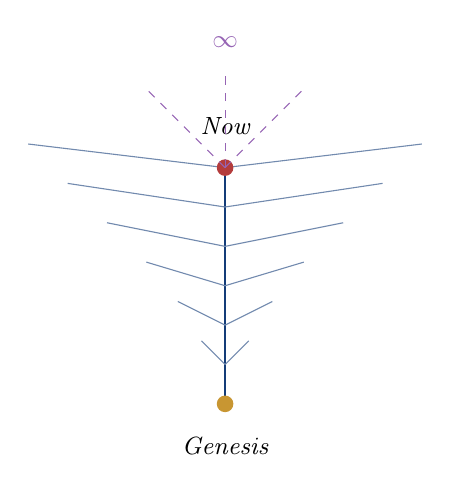
\begin{tikzpicture}
  % The eternal tree
  \draw[thick, deepblue] (0,0) -- (0,3);
  % Branches - the growing past
  \foreach \h/\w in {0.5/0.3, 1.0/0.6, 1.5/1.0, 2.0/1.5, 2.5/2.0, 3.0/2.5} {
    \draw[deepblue!60, thin] (0,\h) -- (-\w, \h+0.3);
    \draw[deepblue!60, thin] (0,\h) -- (\w, \h+0.3);
  }
  % Root - genesis
  \fill[amber] (0,0) circle (3pt);
  \node[below,font=\small\itshape] at (0,-0.3) {Genesis};
  % Tip - the present
  \fill[cosmicred] (0,3) circle (3pt);
  \node[above,font=\small\itshape] at (0,3.3) {Now};
  % Future - open
  \draw[dashed, nebula] (0,3) -- (-1,4);
  \draw[dashed, nebula] (0,3) -- (0,4.2);
  \draw[dashed, nebula] (0,3) -- (1,4);
  \node[above,font=\small\itshape,nebula] at (0,4.4) {$\infty$};
\end{tikzpicture}
\end{center}

% ============================================================================
% References
% ============================================================================
\begin{thebibliography}{99}

\bibitem{qnk-physics} Q-NarwhalKnight Research Group, ``Theoretical Physics of Distributed Consensus: A Quantum Field-Theoretic Framework for DAG-Based Byzantine Agreement,'' Technical Report, February 2026.

\bibitem{qnk-full} Q-NarwhalKnight Development Team, ``Quantum Physics in Q-NarwhalKnight: A Comprehensive Analysis of Quantum-Enhanced Distributed Consensus Systems with String-Theoretic Resonance,'' Whitepaper v3.9, October 2025.

\bibitem{landauer} R. Landauer, ``Irreversibility and Heat Generation in the Computing Process,'' \textit{IBM Journal of Research and Development}, vol. 5, no. 3, pp. 183--191, 1961.

\bibitem{whitehead} A.N. Whitehead, \textit{Process and Reality: An Essay in Cosmology}, Macmillan, 1929.

\bibitem{heidegger} M. Heidegger, \textit{Being and Time} (Sein und Zeit), trans. J. Macquarrie and E. Robinson, Harper \& Row, 1962 [1927].

\bibitem{bergson} H. Bergson, \textit{Time and Free Will: An Essay on the Immediate Data of Consciousness} (Essai sur les donn\'ees imm\'ediates de la conscience), trans. F.L. Pogson, George Allen \& Unwin, 1910 [1889].

\bibitem{leibniz} G.W. Leibniz, \textit{Monadology}, 1714. In R. Ariew and D. Garber, eds., \textit{Philosophical Essays}, Hackett, 1989.

\bibitem{nietzsche} F. Nietzsche, \textit{The Gay Science} (Die fr\"ohliche Wissenschaft), 1882, \S341.

\bibitem{borges} J.L. Borges, ``A New Refutation of Time,'' in \textit{Labyrinths}, trans. J.E. Irby, New Directions, 1962.

\bibitem{mayer} V. Mayer-Sch\"onberger, \textit{Delete: The Virtue of Forgetting in the Digital Age}, Princeton University Press, 2009.

\bibitem{dagknight} Y. Sompolinsky and A. Zohar, ``PHANTOM and GhostDAG: A Scalable Generalization of Nakamoto Consensus,'' IACR ePrint, 2018.

\bibitem{dilithium} L. Ducas et al., ``CRYSTALS-Dilithium: A Lattice-Based Digital Signature Scheme,'' TCHES, 2018.

\bibitem{bulletproofs} B. B\"unz et al., ``Bulletproofs: Short Proofs for Confidential Transactions and More,'' IEEE S\&P, 2018.

\bibitem{parmenides} Parmenides, ``On Nature,'' Fragments B2--B8, c. 475 BCE. In P. Curd, \textit{A Presocratics Reader}, Hackett, 2011.

\bibitem{heraclitus} Heraclitus, Fragments. In C.H. Kahn, \textit{The Art and Thought of Heraclitus}, Cambridge University Press, 1979.

\bibitem{shakespeare} W. Shakespeare, \textit{Sonnets}, 1609.

\bibitem{khayyam} O. Khayy\'am, \textit{Rub\'aiy\'at}, trans. E. FitzGerald, 1859.

\end{thebibliography}

\end{document}
